
\documentclass[journal]{IEEEtran}
\usepackage[cmex10]{amsmath}
\usepackage{amssymb}
\usepackage{mathrsfs}
\usepackage{bm}
\usepackage{dsfont}
\usepackage[pdftex]{graphicx}
% \usepackage[dvips]{graphicx}
\usepackage{graphicx}
\usepackage{subfigure}

\usepackage{cite}
\usepackage{bibentry}
\usepackage{mathtools}
\usepackage{cuted}
\usepackage{xfrac}
\usepackage{multirow}
\usepackage{arydshln}
%\usepackage[dvips]{color}
\usepackage[dvipsnames]{xcolor}


\begin{document}
\title{\textcolor{red}{Optimal coordination of neutral function of directional overcurrent protections for interconnected electric power systems}}

\author{P.~M.~De~Oliveira-De Jesus~\IEEEmembership{Senior Member,~IEEE}, E.~Sorrentino, J.~S.~Abello, O.~Archilla, C.~A.~Alza, \\ D.~F.~Celeita~\IEEEmembership{Senior Member,~IEEE}, G.~A.~Ramos~\IEEEmembership{Senior Member,~IEEE}, A.~J.~Urdaneta~\IEEEmembership{Senior Member,~IEEE}

\thanks{Manuscript received November XX, 20XX}
\thanks{J.~S.~Abello, O.~Archilla, C.~A.~Alza, D.~Celeita, G.~A.~Ramos, and P.\,M.\,De Oliveira-De Jesus are with the Department of Electrical and Electronic Engineering, Universidad de Los Andes, Bogot\'a, Colombia. E-mail: pm.deoliveiradejes@uniandes.edu.co.  A.~J.~Urdaneta is with Simon Bolivar University, Venezuela.
E-mail: alberto@usb.ve, E.~Sorrentino is with Carlos III University, Madrid, Spain.
E-mail: elmer.sorrentino@uc3m.es} % <-this % stops a space
       \thanks{Digital Object Identifier}}

\markboth{IEEE Transactions on Industry Applications,~Vol.~X, No.~X, December~2020}%
{De Oliveira-De Jesus: Transactions onIndustry Applications}

\maketitle
\begin{abstract}
\textcolor{red}{
	  The problem of coordination of directional overcurrent protections (DOCP) in interconnected power systems has been widely treated in literature. Existing procedures are focused on phase 67P function and network models based upon typical positive sequence models. However, the optimal coordination of the neutral 67N function has not been considered. In this paper, we investigate the impact of high-impedance single-phase faults in the  clearing times and selectivity of the 67N function of DOCP whose time dial settings were selected using a standard optimization technique.  
	 The multiphase-multiground (4-wire) network model developed by EPRI for the OpenDSS platform is used to determine the exact fault current distribution across phases, neutrals and the ground path.  As a key contribution, we determine the effect of the fault resistance magnitude on optimal dial settings, overall speed, selectivity and voltage profile for a range of pickup settings. The results show that for a range of pickup settings the optimal operation time decreases as the fault impedance increases until the calculated time dial setting stagnates at the minimum value. Beyond this point, the clearing times reach a minimum and deteriorate as far the fault impedance increases.} 
\end{abstract}


\begin{IEEEkeywords}
directional overcurrent relay coordination, high-impedance faults,  single phase faults, neutral 
\end{IEEEkeywords}

\section{Introduction}

\textcolor{red}{The optimal coordination of directional overcurrent protections (DOCP) in interconnected power systems 
is still a challenging problem.  The first optimization approach to coordinate DOCP was introduced in 1988 by \cite{urdaneta1988} using a linear-programming  approach. The original method was applied to coordinate directional overcurrent function 67 (phase). In this approach optimal relay time dial settings are determined for solid three-phase to ground short-circuit currents \cite{ezzeddine2011coordination}. In the last thirty years a large number of contributions have been proposed to tackle problem resorting to different linear and nonlinear optimization procedures based on 67 phase function and standard positive sequence models.}

\textcolor{red}{The coordination on 67 neutral function DOCP protections have gained great interest since under the smart grid paradigm \cite{jones2013future,ias}. Single-phase faults are very common in medium voltage sub-transmission and distribution systems. These kind of networks are being operated under weakly-meshed schemes in order to improve the power system reliability. So, traditional radial-based operation supported in unidirectional overcurrent protection relays are not longer suitable. The use of directional overcurrent relays to protect meshed networks might be a cost effective alternative.}


 \textcolor{red}{However, the 67N function should be also coordinated accounting the effects of high-impedance phase to earth faults. The optimal coordination  of neutral/earth function of DOCP power systems has been completely overlooked in literature. To do so, we need to determine the magnitude of the asymmetrical faults seen by the 67N function to setup the optimization procedure. A fundamental shortcoming of the short current calculation lies on the use of traditional sequence models disregarding important effects such as mutual couplings, current division at neutral/grounding path and the effect of high-impedance faults. On account of the existence of several short-circuit calculation tools based on multiphase-multiground network models such as the OpenDSS \cite{opendss}, it is now possible to determine precisely how different fault impedance magnitudes change the fault currents and therefore the response of the protection system whose settings were optimized assuming fault currents associated with solid faults. This detailed network model overcomes the limitations of symmetrical components by including the effect of unbalanced loads, neutral grounding through earth resistances and fault impedances
 on short-circuit currents passing through all relays of the system.}

\textcolor{red}{The effect of high impedance faults are critical to ensure speed and selectivity objectives.  Existing optimization procedures cannot answer how high-impedance single-phase to neutral faults affect the optimal clearing time, the selectivity and, the corresponding optimal relay settings. } 

\textcolor{red}{To fulfill the research gap, this paper investigates how different magnitudes of high-impedance faults affect the performance of the protection system. To do so, the proposal is illustrated with the well-known three bus test system introduced by \cite{urdaneta1988} redefined now as a multiphase-mutigrounded network system.}


\textcolor{red}{The paper is organized as follows.  Background  is discussed in Section \ref{background}. The method is presented in Section \ref{theoptmodel}. The case-study is defined in Section \ref{casestudy}. Results are discussed in Section \ref{results}. Conclusions are drawn in Section \ref{conclusions}.}


\section{\textcolor{red}{Background}} \label{background}

\textcolor{red}{Comprehensive reviews of existing optimization procedures can be found in \cite{birla2005time,raza2014optimum} listing around 80 relevant papers on optimal coordination of DOCP from 1988 to 2014. Recently, \cite{godwal2020review} presented an updated review with 23 new papers published between 2014 and 2020.
These review papers classify existing contributions by optimization technique used: linear programming, nonlinear programing and evolutionary optimization.
None of them deal with the problem of how to coordinate the DOCP 67N function and what is the effect
of the single phase to ground fault resistance on speed and selectivity.
In Table \ref{table1} we include the reviews of 2005, 2014 and 2020 as well as a number of recent contributions on optimal coordination of DOCP not included in previous lists.} 

\small
	\begin{table}[!ht]												
	\begin{center}\caption{Summary of existing DOCP optimization procedures}\label{table1}					
	\begin{tabular}{lc|cc|ccc}					
	\hline 	
	
	\small	Reference     &\small year     & \multicolumn{2}{|c|}{\small Relay function}   	&	\multicolumn{3}{c}{ \small Network model}    \\\cline{3-7}	
	
	
	\small	 		&	    & 67P & 67N & + seq. & 3phase&4wire \\\hline
\scriptsize Review paper \cite{birla2005time}    &2005&$\circ$& &$\circ$ &&\\	
\scriptsize Review paper \cite{raza2014optimum}  &2014&$\circ$& &$\circ$ &&\\
\scriptsize Review paper \cite{godwal2020review} &2020&$\circ$& &$\circ$ &&\\
\scriptsize \cite{sorrentino2020novel}          &2020&$\circ$& &$\circ$ &&\\
%\scriptsize 	\cite{	el2020improved		}    &2020&$\circ$& &$\circ$ &&\\	
%\scriptsize 	\cite{	chheng2020coordination		}    &2020&$\circ$& &$\circ$ &&\\	
%\scriptsize 	\cite{	korashy2020developed		}    &2020&$\circ$& &$\circ$ &&\\	
\scriptsize 	\cite{	ghotbi2020determination		}    &2020&$\circ$& &$\circ$ &&\\	
\scriptsize 	\cite{	sulaiman2020plant		}    &2020&$\circ$& &$\circ$ &&\\	
\scriptsize 	\cite{	shah2020new		}    &2020&$\circ$& &$\circ$ &&\\	
\scriptsize 	\cite{	gupta2020optimal		}    &2020&$\circ$& &$\circ$ &&\\	
\scriptsize 	\cite{	korashy2020optimal		}    &2020&$\circ$& &$\circ$ &&\\	
\scriptsize 	\cite{	darabi2020dual		}    &2020&$\circ$& &$\circ$ &&\\	
\scriptsize 	\cite{	dawood2020optimum		}    &2020&$\circ$& &$\circ$ &&\\	
\scriptsize 	\cite{	mahboubkhah5modified		}    &2020&$\circ$& &$\circ$ &&\\	
\scriptsize 	\cite{	mokhtarpourperformance		}    &2020&$\circ$& &$\circ$ &&\\	
\scriptsize 	\cite{	fatemi2020considering		}    &2020&$\circ$& &$\circ$ &&\\	
\scriptsize 	\cite{	kamel2020development		}    &2020&$\circ$& &$\circ$ &&\\	
\scriptsize 	\cite{	damchi2020hybrid		}    &2020&$\circ$& &$\circ$ &&\\	
\scriptsize 	\cite{	kida2020improved		}    &2020&$\circ$& &$\circ$ &&\\	
\scriptsize 	\cite{	samadi2020adaptive		}    &2020&$\circ$& &$\circ$ &&\\	
\scriptsize 	\cite{	alaee2020optimal		}    &2020&$\circ$& &$\circ$ &&\\	
\scriptsize 	\cite{	saldarriaga2020optimal		}    &2020&$\circ$& &$\circ$ &&\\	
\scriptsize 	\cite{	sadeghi191optimal		}    &2020&$\circ$& &$\circ$ &&\\	
\scriptsize 	\cite{	sarwagya2020optimal		}    &2020&$\circ$& &$\circ$ &&\\	
\scriptsize 	\cite{	sorrentino191efficient		}    &2020&$\circ$& &$\circ$ &&\\	
\scriptsize 	\cite{	mahboubkhah2020considering		}    &2020&$\circ$& &&$\circ$ &\\	
\textbf{This paper}	                                       &-&       &$\circ$& &&$\circ$\\
	\hline	
\end{tabular}												
\end{center}												
\end{table}
\normalsize

\textcolor{red}{In general, the coordination of 67 function at transmission level uses the positive sequence model\cite{	el2020improved		}-\cite{	kida2020improved		}. 
Notice that \cite{samadi2020adaptive,alaee2020optimal,saldarriaga2020optimal,	sadeghi191optimal,
	sarwagya2020optimal,sorrentino191efficient,mahboubkhah2020considering} describe some applications
	in distribution systems. However, despite the distribution system is general untransposed with asymmetrical primitive matrices, the coordination of the 67 phase function is carried out using positive network sequence models. It is interesting to mention that \cite{mahboubkhah2020considering} solves the problem  of coordination of 67P relays by means of a real-time platform based upon a three-phase model. In this review, no evidence of optimal coordination of neutral DOCP with multi-phase multi-ground network model has been found.}

 
 \section{Method} \label{theoptmodel}

The original optimization problem was written to coordinate  67 phase relays considering solid three-phase faults \cite{urdaneta1988}. This method is now adapted to perform optimal coordination of 67N relays in meshed systems when different fault impedances (not only solid faults) occurs in the system affecting speed and selectivity.

\subsection{Assumptions}

Real-wold power systems are complex and for the sake of simplicity the following assumptions and limitations are considered in the formulation of the optimization problem.


\begin{enumerate}

\item The optimization problem is posed by assuming that the magnitude of the fault impedance is the same for all possible "relevant" faults located at near and end terminal of each line, just as the standard model \cite{urdaneta1988} assumes that all relevant faults are solid, that is $R_F$=0. The use of a unique fault impedance magnitude for all faults of the model is debatable in account of its stochastic nature. It is clear that the coordination problem must be solved for the expected fault impedance magnitude and the corresponding variances. However, if we account the fault impedance magnitude as a probability function, the approach turns the model into a stochastic optimization problem. The stochastic view of this problem is out of scope.


\item All asymmetrical phase-to-neutral faults were produced at same phase. In this case we select phase $c$ (the nearest to ground).

\item Transient configurations are not included in the optimization problem formulation. In real-world the relaying system does not operate at the same time. Thus, the short circuit current magnitude seen by each relay adopts different values owing to topology changes. Despite this problem has been solved in \cite{urdaneta1997optimal,sorrentino2020novel}, this aspect has been overlooked in all existing DOCP optimization. The main consequence of disregard transient configurations lies on increased sensitivity problems in backup relays due to unrealistic low fault currents.

   \item The use of the OpenDSS tool to determine fault currents include prefault conditions. However. in this paper we neglect load currents, neither balanced nor balanced.

   \item We assume that the sensitivity problem is solved. In this paper we assume all relays are adjusted with the same pick-up currents of the 67N function. In general this value is set between 10 \% of the current transformer capacity and 80 \% of minimum short circuit current.

  \item Short-circuit current magnitudes are assumed as invariant values over time. The effect of decrement factors are not included.

  \item Only time-delayed relays are considered.  The coordination time is unique for all primary-backup pairs. The effect of time-definite adjusts are out of scope.

\item Circuit breaker operation times are not included in the model.

  \item Only standard curves are considered, and all the relays are assumed to be with the same curve.

  \item Equivalent impedances at source buses are assumed the same at peak and off-peak load. Thus, the fault currents do not change along the time.

\item Resistance of all ground mats at substations are equal to zero.

\item The optimization model is built considering that near-end and far-end Faults occur at substations.

\item Influence of stability constraints is not considered.

\end{enumerate}




 
 
 
\subsection{Problem formulation}

 Consider a meshed power system with $k$=1,...,$n_l$ three-phase transmission lines. The set of transmission lines is defined as $k\in \mathds{N}$ with $n_l=\dim{(\mathds{N})}$. Each line has two overcurrent 67N relays. Thus, a  total of $r$=1,$\ldots$, $n_r$=2$n_l$ relays are installed in the system. The set of relays is defined as $r\in \mathds{R}$ with $n_r=\dim{(\mathds{R})}$. Each relay  $r\in \mathbf{R}$ is characterized by the following manner. Current-time curve parameters for each relay are fixed and defined by three parameters: $\alpha_{r1}\in \bm {\alpha}$,  $\alpha_{r2}\in \bm {\alpha}$ and $\alpha_{r3}\in \bm {\alpha}$. Pick-up currents $I_{pr} \in \bm {P}$
 depend on maximum unbalanced currents that may flow by the line, and  the time dial setting $D_r\in \bm {D}$ are defined by the protection engineer according to a coordination criteria.
\begin{figure}[t] \centerline{
     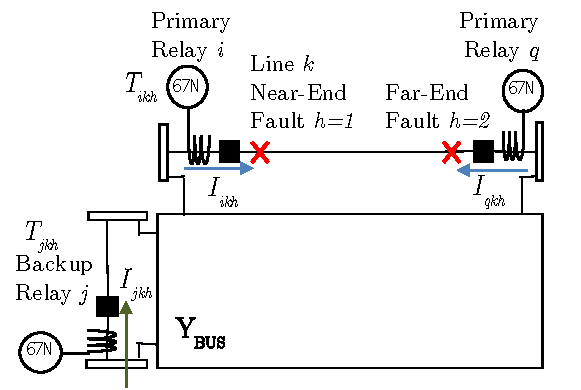
\includegraphics[width=2.3in]{images/main-backup.pdf}}
       \caption{Primary-backup relays}
      \label{main}
        \end{figure}

Figure \ref{main} shows a faulted line $k\in \mathbf{N}$. Line $k$ is protected by two primary  67N overcurrent relays $i\in \mathds{R}$ and $q\in \mathds{R}$. Depending on the network topology, we can identify a number of relays pairs (primary relay $i\in \mathds{R}$ and backup relay $j\in \mathds{R}$) that must be coordinated.
The set of "relevant" faults is defined as $h\in \mathds{H}$ with $n_f=\dim{(\mathds{H})}$ the number of faults under consideration. We identify two relevant faults per line $k$, $\mathds{H}$=$\{1,2\}$. Thus, $n_f$=2. A near-end fault ($h$=1) whose location is closer to relay $i$ and a near-far fault ($h$=2) adjacent to relay $q$. Given a fault $h\in \mathds{H}$ over the line $k$, if a primary relay $i$ does not clear the fault, another adjacent (backup) relay $j$ (located in other adjacent line) should clear the fault. All relays of the system can operate as primary or backup depending on whether the fault is located in its own line or the fault is located in adjacent line.


Figure \ref{main} shows the situation when both primary relays $i$ and $q$  operate successfully when a fault $h$ occurs in line $k$. In this case, each primary-backup relay-pair $i-j$ must fulfill the following inequality time operation constraint:


\begin{equation} \label{SCTstat}
  T_{jkh}-T_{ikh}\geq C\quad i,j\in \mathds{R}, k\in \mathds{N}, h\in \mathds{H}
\end{equation}

where $T_{ikh}$ is a primary  operating time (for a relay $i$ located in the line $k$ with fault $h$),  $T_{jkh}$ is a backup operating time (for a relay $j$ located in an adjacent line of the line $k$ with fault $h$, not in the same line), and $C$ is a known value, the coordination time specified by the protection engineer for all primary-backup pairs.





The operation time for the primary relay $i$ when the fault $h$ occurs at line $k$ is expressed as:

\begin{equation}\label{primary}
  T_{ikh}=\frac{\alpha_{i1} D_{i}}{(\frac{I_{ikh}}{I_{pi}})^{\alpha_{i2}}+\alpha_{i3}}=\beta_{ikh}D_{i}
\end{equation}

where single-phase short-circuit current contribution seen by a relay $i$ due to fault $h$ at line $k$ ($I_{ikh}$) must be determined using the primitive admittance matrix $Y_{BUS}$ with all breakers of the system closed. The maximum multiplier allowed is $M^{max}$=$\frac{I_{ikh}}{I_{pi}}$=30. For short-circuit $I_{ikh}$ currents higher than $30{I_{pi}}$, the operation time is constant  $T_{ikh}$=$\frac{\alpha_{i1} D_{i}}{30^{\alpha_{i2}}+\alpha_{i3}}$.

Likewise, the  operation time for the backup relay $j$ when the fault $h$ occurs at line $k$ is expressed as:

\begin{equation}\label{primaryxx}
  T_{jkh}=\frac{\alpha_{j1} D_{j}}{(\frac{I_{jkh}}{I_{pj}})^{\alpha_{j2}}+\alpha_{j3}}=\beta_{jkh}D_{j}
\end{equation}

where single-phase short-circuit current contribution seen by a relay $j$ due to fault $h$ at line $k$ ($I_{jkh}$) must be determined using the primitive admittance matrix $Y_{BUS}$ with all breakers of the system closed. Thus, given a fault $h$ at line $k$ both adjacent relay operation times can be expressed as a function of relay curve parameters and pick-up currents. Primary operation time  $T_{ikh}$=$\beta_{ikh}D_{i}$ where $\beta_{ikh}$=${\alpha^{-1}_{i1}}{[(\frac{I_{ikh}}{P_{i}})^{\alpha_{i2}}+\alpha_{i3}]}$ must be lower than the backup operation time $T_{jkh}$=$\beta_{jk}D_{j}$ where $\beta_{jkh}$=${\alpha^{-1}_{j1}}{[(\frac{I_{jkh}}{P_{j}})^{\alpha_{j2}}+\alpha_{j3}]}$. Therefore, Eq. \ref{SCTstat} can be rewritten as:

 \begin{equation} \label{SCTstat2}
  \beta_{jkh}D_{j}-\beta_{ikh}D_{i}\geq C\quad  i,j\in \mathds{R}, k\in \mathds{N}, \mathds{H}=\{1,2\}
\end{equation}

where $C$ is the predefined coordination time. Normal load and short circuit currents are sensed by neutral directional overcurrent functions 67N through the sum of three phase currents measured by current transformers at phases or a by  a separate current transformer for grounded neutrals at each substation.

Linear factors $\beta_{ikh}$ and  $\beta_{jkh}$   should be determined considering two feasible single-phase faults located at near-end ($h$=1) and far-end of line $k$=1,...,$n_l$. In many cases the use on near-end and near-far fault locations as relevant faults are sufficient to ensure complete selectivity. However, if transient configurations during the clearing time process are duly considered, the set of relevant faults that ensure complete selectivity must be previously determined in order to formulate an optimization model that assures full selectivity. The inclusion of transient configurations is out of scope of this paper.


It is important to stress out that  $\beta_{ikh}$  factors depend on single-phase to neutral short circuit magnitudes $I_{ikh}$  whose magnitudes are strongly dependent upon the grounding path. Fault current $I_{ikh}$ can be determined using a detailed network model such as EPRI's NEV OpenDSS platform.

Optimization problem constraints can be now defined for a generalized system with $n_l$ lines, $n_r$ relays and $n_f$=2 feasible fault locations. A total of $n_b$ feasible primary-backup pair constraints must be identified and grouped in this compact form:

\begin{equation}\label{BB}
 \mathbf{S}=\mathbf{B}\cdot\mathbf{D}\ge C\mathbf{u}
\end{equation}

where $\mathbf{S}$ is the separation times vector,  $\mathbf{D}$ is the $n_r$ dimension vector with the time dial of each relay and $\mathbf{B}$ is the   coordination matrix that depends on linear factors $\beta_{ikh}$  and $\beta_{jkh}$ for $h$=1,2. The coordination matrix $\mathbf{B}$ has $n_r$ columns and $n_b$ rows. The number of rows will depend on the number of effective primary-backup pairs. Entry  $\mathbf{u}$ is a $n_b$ row unit vector and $C$ is the specified coordination time between primary and backup relays.

The objective function (OF) of the optimization problem is defined as the average sum of operating times of all the
primary relays for the two faults ($n_f$=2), near-end and far-end faults under consideration:

\begin{equation}\label{objective}
  \mbox{OF}=\frac{1}{n_f}\sum_{h=1}^{n_f}\sum_{k=1}^{n_l}\sum_{i=1}^{n_r}m_{ik}  T_{ikh}
\end{equation}


where $m_{ik}$ is equal to 1 if the primary relay $i$ is located at line $k$, otherwise  $m_{ik}$=0.


Finally, once the objective function and the corresponding constraints are duly defined, the optimization problem is stated as follows.
For a given the system data (primitive admittance matrix) and relay data (current-time parameters and pickup currents) determine the best set of time dial settings ($\mathbf{D^*}$) that minimizes the overall system primary relay operation time (OF) considering selectivity constraints. 

\begin{eqnarray}\label{odocr1}
& &  \min_{\mathbf{D^*}} \quad \mbox{OF}=\frac{1}{n_f}\sum_{h=1}^{n_f}\sum_{k=1}^{n_l}\sum_{i=1}^{n_r}m_{ik}  T_{ikh}  \\ \nonumber
& & \mbox{subject to}:\\\label{odocr2}
& &\mathbf{S}=\mathbf{B}\cdot\mathbf{D}\ge C\mathbf{u}\\\label{odocr3}
& &\mathbf{D}\le\mathbf{D^{max}}\\\label{odocr4}
& &\mathbf{D}\ge\mathbf{D^{min}}
\end{eqnarray}

where  $\mathbf{D^{min}}$ and $\mathbf{D^{max}}$ are the dial limits vectors.
The optimization problem has $n_r$ unknowns. The maximum number of inequality restrictions will be 4$n_l$ if all pairs primary-backup relays are able to detect the magnitude and/or direction of the fault.
The above stated optimization problem is suitable to be solved using any linear programming tool, such as Matlab's LinProg.


In this paper, we investigate how  the optimal settings ($\mathbf{D}$), the resulting operation time  (objective function $OF$) and separation times ($\mathbf{S}$) are affected when the coordination matrix ($\mathbf{B}$) is calculated using different high-impedance phase to neutral fault conditions. To do so, single-phase short-circuit currents $I_{ikh}$ and $I_{jkh}$ are calculated using a multiphase-multiground model considering different fault resistances $R_f$ \cite{ias}.

 \section{Test system}  \label{casestudy}

\begin{figure}[t!] \centerline{
     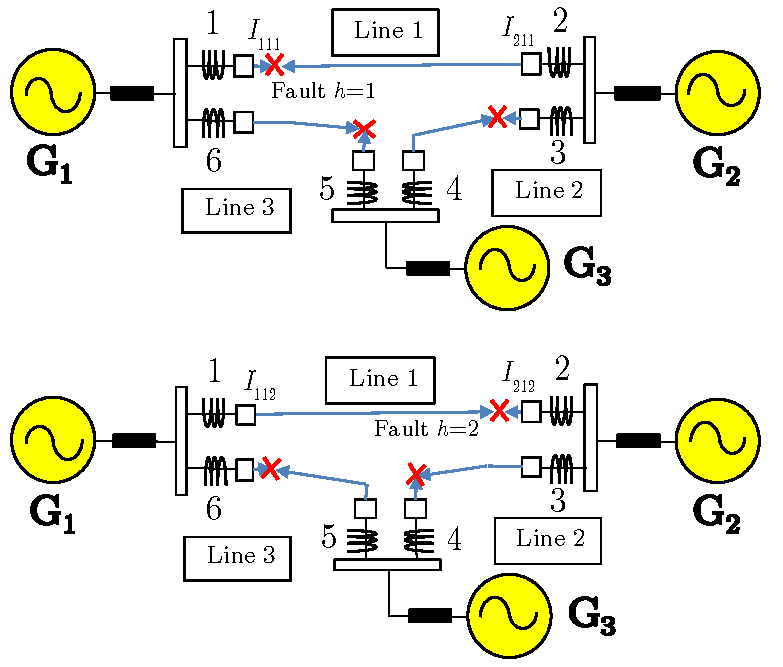
\includegraphics[width=6.4cm]{images/figure1.pdf}}
       \caption{Test system - One-line diagram and fault locations\cite{urdaneta1988}}
      \label{figure1}
        \end{figure}

                 \begin{figure*}[t!] \centerline{
     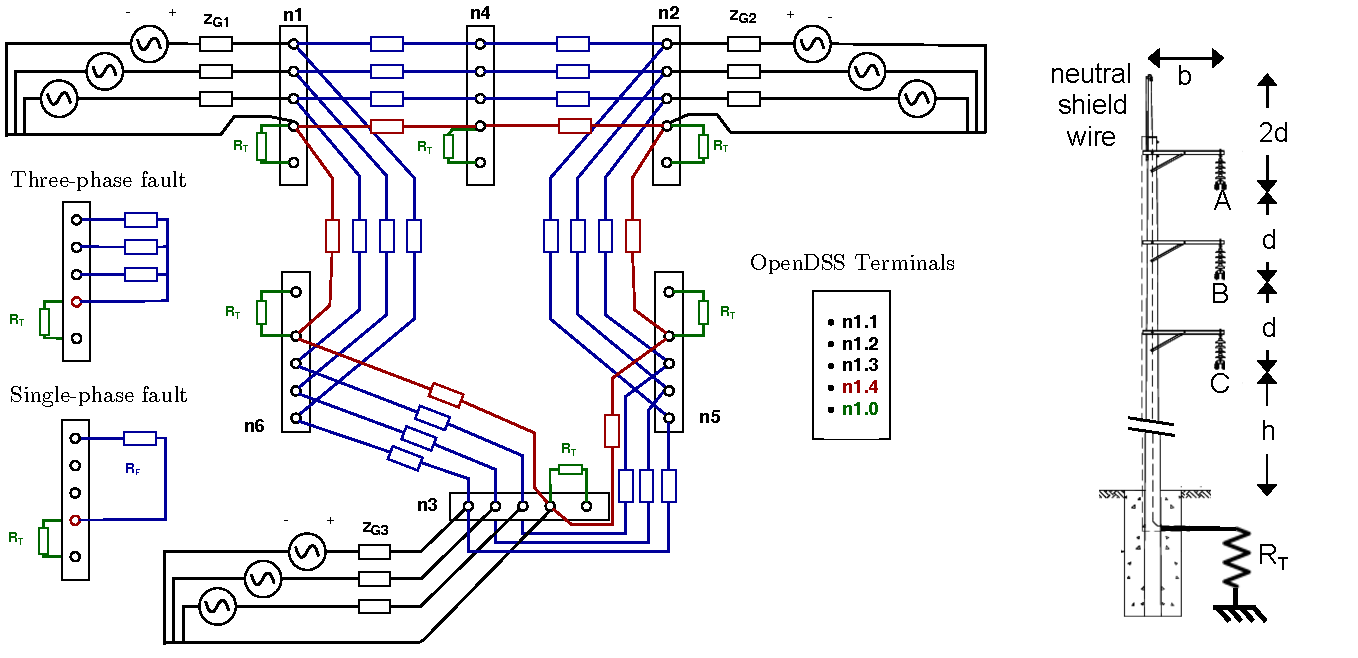
\includegraphics[width=12.0cm]{images/figure2.pdf}}
       \caption{Test system - Multi-phase Multi-ground diagram and tower sketch}
      \label{figure2}
        \end{figure*}



The classic formulation was originally applied over the test-system depicted in Fig. \ref{figure1} considering three-phase faults and the coordination of six relays 67P.
The original test system comprises three substations, three generators with reactance $X^+_1$ = $X^-_1$ = $X^0_1$ = 20  \% (100 MVA), $X^+_2$ = $X^-_2$ = $X^0_2$ = 12 \% (25 MVA) and $X^+_3$ = $X^-_3$ = $X^0_3$ = 18 \% (50 MVA). Positive sequence series impedance of the three lines are:
 $Z^+_1$ = 5.5 + j 22.85 $\Omega$ (50km), $Z^+_2$ = 4.4 + j 18.00 $\Omega$ (40km) and $Z^+_3$ = 7.6 + j 27.00 $\Omega$ (60km). The system has no loads.
  67N phase relay parameters are $\alpha_{i1}$ = 0.14, $\alpha_{i2}$ = 0.02, $\alpha_{i3}$ = -1 for $i$ = 1,...,6 (standard inverse curve). All pick-up currents were set 50A.

Positive sequence impedance parameters for lines and generators are given above in order to determine three-phase short-circuit currents required by  67 (phase) relays to operate. However, in order investigate how to optimize the coordination of  67N (neutral) relays we need to determine exact short-circuit currents for single phase $c$ to neutral faults. To do so, we must build an equivalent 4-wire model for the original positive sequence model provided in \cite{urdaneta1988}  by scripting a new multi-phase multi-ground model under the OpenDSS platform \cite{opendss}.

Figure \ref{figure2} shows the multiphase diagram equivalent for the one-line diagram depicted in Fig. \ref{figure1}. The OpenDSS tool provides an explicit network representation for all system elements.
Besides  three-phases represented in blue color, system neutrals (shield wires) and ground resistances $R_T$ are highlighted in red color and green colors, respectively. Single-phase to neutral faults are represented by $R_F$. For instance, a single-phase $c$ to neutral fault with $R_F$=100 $\Omega$ in line 1 is coded as: \scriptsize
 \texttt{New fault.1   Bus1= n4.3   Bus2=n4.4 r=100}. \normalsize


\begin{table}[t]
\begin{center}\caption{Tower/pole geometry sketch}\label{Table2}
\centering
\begin{tabular}{lccccc}\hline
Line & $d$ (ft)  & $b$ (ft) & $h$ (ft) & Phase conductor & Neutral  \\\hline
1-2  & 7.85 & 6.0      &  40 & 500MCM Conlay AA & ACSR 4/0 6/1\\
2-3  & 9.70 & 5.0      &  40 & 605MCM 54/7 ACSR & ACSR 4/0 6/1\\
3-1  & 10.6 & 5.5      &  40 & 605MCM 54/7 ACSR & ACSR 4/0 6/1\\\hline
\end{tabular}
\end{center}
\end{table}

\begin{table}[t]
\begin{center}\caption{Phase \& neutral conductor characteristics}\label{Table3}
\centering
\begin{tabular}{lccc}\hline
Type & Size & Resistance (ohm/mile)  & GMR (ft)  \\\hline
ACSR 6/1 & 4/0 AWG  & 0.5920 & 0.00814 \\
AA Conlay & 500 MCM & 0.2023 & 0.02600 \\
ACSR 54/7 &605 MCM&0.1756 &0.03210\\\hline
\end{tabular}
\end{center}
\end{table}


        
Primitive impedance matrices  for lines and generators must be provided. Transmission lines primitive matrices are get from the tower sketch shown in Fig. \ref{figure2}
 with dimensions provided in Table \ref{Table2}. Phase conductor characteristics are given in
Table  \ref{Table3}. Transmission line positive sequence impedances for the tower structure depicted in   Fig. \ref{figure2} coincides with the ones specified in the original three-bus test case \cite{urdaneta1988}.






The case-study shown in Fig. \ref{figure2} has six buses. Buses 1, 2 and 3 correspond to generating substations and buses 4, 5 and 6 correspond to a faulted point at given distance from substation $k$, for $k$=1,2,3. In this paper, we only use near-end and near-far faults as seen in  Fig. \ref{figure1}. Thus, the distance of all faults from substations is set equal to 1 meter.


The six bus system depicted in  \ref{figure2} was scripted in OpenDSS. Short-circuit impedances of generators are provided under a three-phase base coinciding with the original ones.




  \section{Results}  \label{results}

The problem solution approach is described in detail so that the interested reader can easily replicate the results with the script included in the following GitHub page:  https://github.com/pmdeoliveiradejesus/Optimal-67N-DOCR-coordination. Optimization was performed in Matlab using the LinProg optimization tool. Fault currents were acquired from the OpenDSS using the COM interface. Specific cases were also coded and solved with MS Excel's solver tool for illustrative purposes.


  The proposed optimization model was applied to the case-study described in Section \ref{casestudy}.
    The case study has $n_l$ = 3, $\mathds{N}$=\{1,2,3\}, lines and $n_r$ = 6 relays,
      $\mathds{R}$=\{1,2,3,4,5,6\}. Two faults ($n_f$=2) are modelled.


      Two scenarios are analyzed:
\begin{enumerate}
  \item Case 1: Faults at near-end and far-end of all lines with $R_F$=0 $\Omega$
  \item Case 2: Faults at near-end and far-end of all lines with $R_F$=10.0 $\Omega$
\end{enumerate}

Finally a sensitivity analysis is carried out varying $R_F$  from 0  $\Omega$ to 50  $\Omega$  when the optimization problem becomes not-well defined due to low currents make the relay system insensible.

A total of $n_b$ = 12 primary-backup ($ikh$-$jkh$) pairs are identified. The fault currents ($I_{ikh}$ and $I_{jkh}$) determined using the OpenDSS 4-wire model and the corresponding $\beta$-factors ($\beta_{ikh}$ and $\beta_{jkh}$) for both scenarios can be found in \cite{ias}. Notice that some primary-backup ($ikh$-$jkh$) pairs have currents with opposite directions (631-231,
112-512,  532-332). In case 1 and case 2 some  $\beta$-factors
are negative. This means the existence of short-circuit contributions lower
that the selected pick-up currents (50A).  In case 1 all short-circuit contributions are greater
that the selected pick-up currents except primary-backup ($ikh$-$jkh$) pairs 211-411 and 112-512.
In  case 2, primary-backup ($ikh$-$jkh$) pairs 211-411,
421-621,631-231 do not operate for near-end faults and relay pairs 112-512, 322-122, 532-332 do not operate for far-end faults. It is clear that as in case 2 $R_F$ is not solid some loss of sensitivity is observed.

  The general optimization model is given by the minimization of sum of all primary times when the fault occurs at near-end and near-far of each line of the system constrained to the coordination equation and corresponding time delay setting limits as follows:

\scriptsize

\begin{equation}\label{Bm}
   \min_{\mathbf{D^*}}\quad \beta_{111}D_1+\beta_{212}D_2+\beta_{321}D_3+\beta_{422}D_4+\beta_{531}D_5+\beta_{632}D_6
\end{equation}


\begin{eqnarray}   \label{opt2}
&&\mbox{subject to}:\\\nonumber
&&  \begin{bmatrix}
    -\beta_{111}    &   0   &   0   &   0   &   \beta_{511} &   0   \\
    \beta_{121} &   0       &   -\beta_{321}    &   0   &   0   &   0   \\
  0&  0       &   \beta_{331} &   0   &   -\beta_{531}    &   0   \\
  0&  -\beta_{211}        &   0   &   \beta_{411} &   0   &   0   \\
0&  0       &   0   &   -\beta_{421}    &   0   &   \beta_{621} \\
0&  \beta_{231}     &   0   &   0   &   0   &   -\beta_{621}    \\
    -\beta_{112}    &   0   &   0   &   0   &   \beta_{512} &   0   \\
    \beta_{122} &   0       &   -\beta_{322}    &   0   &   0   &   0   \\
  0&  0       &   \beta_{332} &   0   &   -\beta_{532}    &   0   \\
  0&  -\beta_{212}        &   0   &   \beta_{412} &   0   &   0   \\
0&  0       &   0   &   -\beta_{422}    &   0   &   \beta_{622} \\
0&  \beta_{232}     &   0   &   0   &   0   &   -\beta_{622}    \\
  \end{bmatrix}
  \begin{bmatrix} \nonumber
  D_1\\D_2\\D_3\\D_4\\D_5\\D_6\\
  \end{bmatrix}
\ge  \begin{bmatrix} \nonumber
  C\\C\\C\\C\\C\\C\\
  \end{bmatrix}\\\nonumber
& & 0.1\le{D_i}\quad i=1...6\\\nonumber
 \end{eqnarray}
\normalsize

The coordination matrix $\mathbf{B}$ is given by Eq. \ref{BB}. As some primary-backup ($ikh$-$jkh$) pairs
 do not operate due to
selectivity and sensitivity problems, the size of $\mathbf{B}$ changes since  rows corresponding to conflictive
primary-backup pairs should be eliminated. 


\subsection{Case 1: solid fault}\label{1}

 According to the calculated fault currents and linear factors \cite{ias} and the formulation given in Eq. \ref{opt2}, the resulting optimization model for solid faults (with $R_F$ = 0) is:
 
\scriptsize
\begin{equation}\nonumber
   \min_{\mathbf{D^*}}\quad 2.30 D_1+2.45  D_2+2.30  D_3+2.25  D_4+ 2.54  D_5+2.43 D_6
\end{equation}

\begin{eqnarray}\nonumber
&&\mbox{subject to}:\\\nonumber
&&  \begin{bmatrix}
-1.99	&	0.00	&	0.00	&	0.00	&	3.10	&	0.00	\\
2.63	&	0.00	&	-1.99	&	0.00	&	0.00	&	0.00	\\
0.00	&	0.00	&	2.62	&	0.00	&	-1.99	&	0.00	\\
0.00	&	0.00	&	0.00	&	-2.53	&	0.00	&	31.45	\\
8.74	&	0.00	&	-2.62	&	0.00	&	0.00	&	0.00	\\
0.00	&	-1.99	&	0.00	&	2.53	&	0.00	&	0.00	\\
0.00	&	0.00	&	0.00	&	-1.99	&	0.00	&	2.89	\\
0.00	&	2.92	&	0.00	&	0.00	&	0.00	&	-1.99	\\
  \end{bmatrix}
  \begin{bmatrix} \nonumber
  D_1\\D_2\\D_3\\D_4\\D_5\\D_6\\
  \end{bmatrix}
\ge  \begin{bmatrix} \nonumber
  0.2\\0.2\\0.2\\0.2\\0.2\\0.2\\
  \end{bmatrix}\\\nonumber
& &{D_i}\ge0.1\quad i=1...6\\\nonumber
 \end{eqnarray}
\normalsize

  The solution for the optimal clearing time for faults with $R_F$=0 is OF= 3.6551s. The resulting optimal time dial settings are   $D_1$=0.2711,
    $D_2$=0.2427,
    $D_3$=0.2579,
    $D_4$=0.2703,
    $D_5$=0.2387 and,
    $D_6$=0.2553. It is worth to note that separation times (given by $\mathbf{B}\cdot \mathbf{D}$) are equal to the prescribed coordination time (0.2s) with two exceptions  in rows 4 and 5 of the coordination matrix: -2.53$D_4$+31.45$D_6$=7.34s and   8.74$D_1$-2.62$D_4$=1.69s.


        \textcolor{red}{\textbf{Validation of results}: the overall operation time and selectivity of the protection system is simulated  by inserting 5000 random-located faults in the transmission system.
         Figure 4(a) shows a histogram with the distribution of primary operation times (Eq. \ref{odocr1}) for the resulting optimal time dial settings reported above for solid faults. The average time is 3.3511s with standard deviation
 0.0780s. The distribution of separation times (Eq. \ref{odocr1})   is  presented in the histogram shown in Fig. 4(b). Observe that there is no separation time is below the predefined coordination time interval (C =200ms). A histogram with resulting voltages in all phases is also depicted in  Fig. 5(a)}. No temporary overvoltages are observed when solid faults are inserted. 
 
         \begin{figure}[t!] \centerline{
     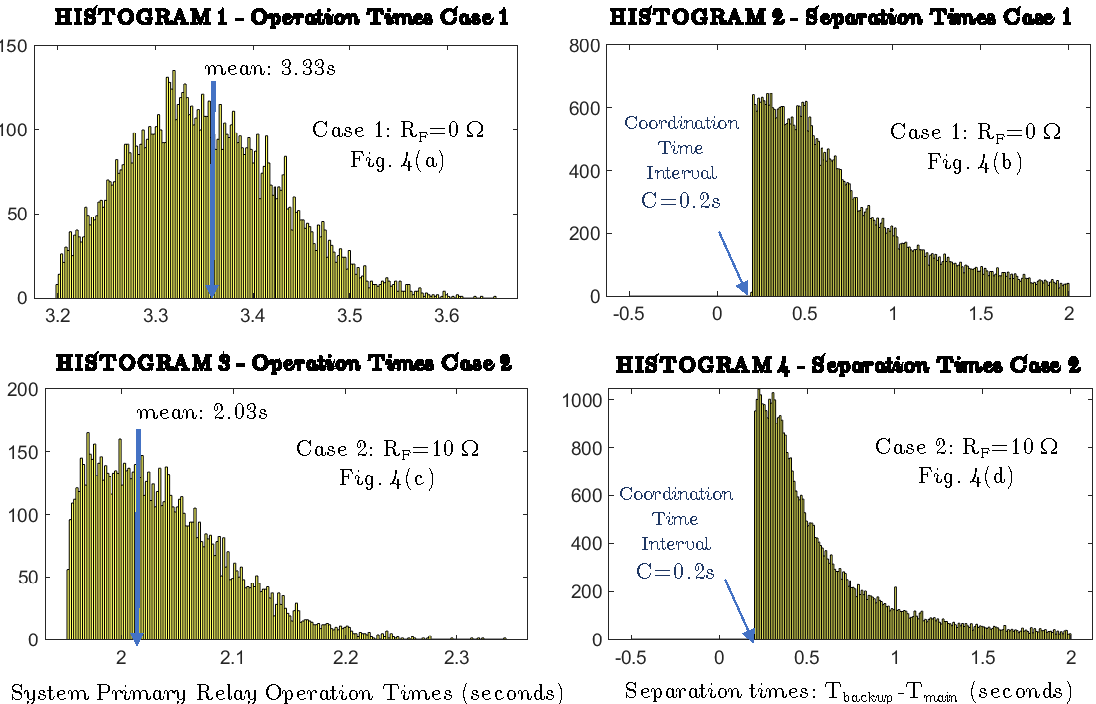
\includegraphics[width=9cm]{images/val1.pdf}}
       \caption{Test system - speed and selectivity in Cases 1 and 2}
      \label{figure5x}
        \end{figure}
        
               
 \begin{figure}[t!] \centerline{
     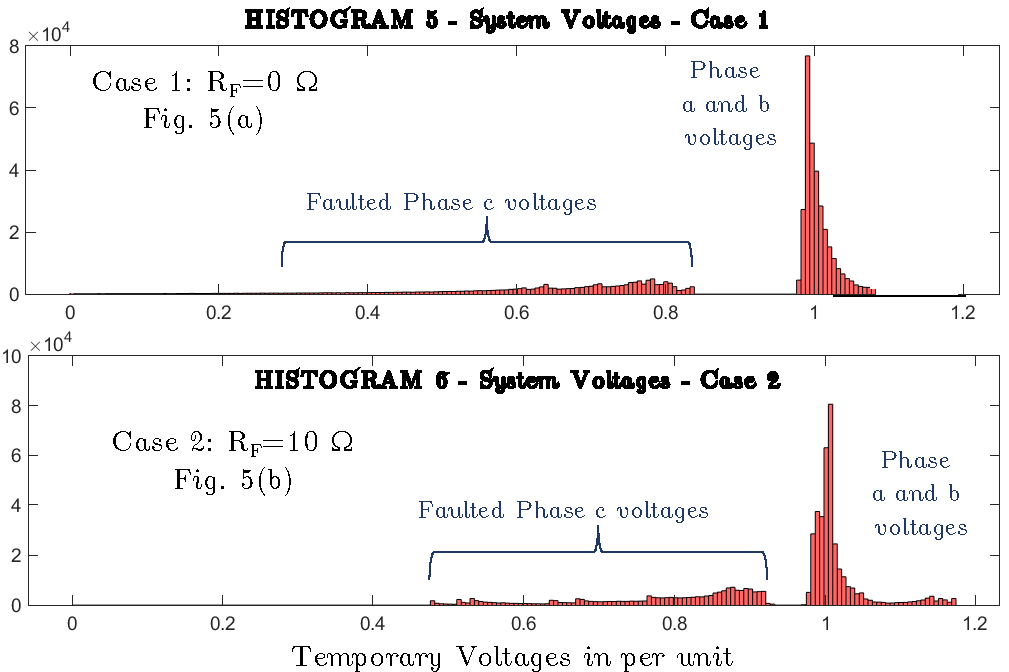
\includegraphics[width=8.7cm]{images/val2.pdf}}
       \caption{Test system - Temporary overvoltages in Cases 1 and 2}
      \label{figure6x}
        \end{figure}
        
\subsection{Case 2: $R_F$ = 10 $\Omega$}\label{2}
\normalsize
  The resulting optimization model for  a non-solid fault, $R_F$ = 10 $\Omega$  is given by:
\scriptsize
\begin{equation}\nonumber
   \min_{\mathbf{D^*}}\quad 2.01 D_1+2.23   D_2+2.25  D_3+2.17  D_4+ 2.14   D_5+2.67 D_6
\end{equation}

\newpage 
\begin{eqnarray}\nonumber
&&\mbox{subject to}:\\\nonumber
&&  \begin{bmatrix}
-1.99	&	0.00	&	0.00	&	0.00	&	4.18	&	0.00	\\	
3.03	&	0.00	&	-1.99	&	0.00	&	0.00	&	0.00	\\	
0.00	&	0.00	&	3.07	&	0.00	&	-1.99	&	0.00	\\	
16.71	&	0.00	&	-3.07	&	0.00	&	0.00	&	0.00	\\	
0.00	&	-1.99	&	0.00	&	2.89	&	0.00	&	0.00	\\	
0.00	&	0.00	&	0.00	&	-1.99	&	0.00	&	3.46	\\	
0.00	&	3.86	&	0.00	&	0.00	&	0.00	&	-1.99	\\	

  \end{bmatrix}
  \begin{bmatrix} \nonumber
  D_1\\D_2\\D_3\\D_4\\D_5\\D_6\\
  \end{bmatrix}
\ge  \begin{bmatrix} \nonumber
  0.2\\0.2\\0.2\\0.2\\0.2\\0.2\\
  \end{bmatrix}\\\nonumber
& &{D_i}\ge0.1\quad i=1...6\\\nonumber
 \end{eqnarray}
\normalsize

Notice that only seven relays are capable to detect the fault current.  Three rows coordination matrix should be also removed since some backup fault currents are going in the opposite direction and two rows correspond to a negative operation time.

The optimal clearing time obtained 2.3222s. Notice that this time is lower than the one obtained in previous case 1 and the optimal settings are:
$D_1$=0.1617,
$D_2$=0.1282,
$D_3$=0.1457,
$D_4$=0.1572,
$D_5$=0.1247
, and $D_6$=0.1484. 


\textcolor{red}{\textbf{Validation of results}: as done in case 1 we insert 5000 random-located faults with a resistance of 10 ohms $\Omega$ to determine statistical distribution of operation and separation times considering now the optimal dial settings obtained in case 2. The
 histogram shown in Fig. 4(c) indicates that  the mean operation time is  2.0353s with standard deviation
 0.0589s.   
  Resulting relay operation time associated to optimal settings of case 2 with $R_F$=10 $\Omega$ is lower than the one obtained with settings of case 1 with $R_F$=0  $\Omega$. This means that betters results can be obtained if non-solid faults are considered. We must stress that current optimization procedures neglect the effect of the fault resistance magnitude. Finally, the distribution of separation times for settings obtained in case 2 are
   depicted in the histogram shown in Fig. 4(d). In this case we also observe full selectivity. No separation time is below 200ms. The inclusion of a fault resistance does not affect the selectivity. A histogram with resulting voltages is depicted in Fig. 5(b). Higher voltages are observed but none exceeds 1.2 pu.}

 \newpage 
\subsection{Verification with non-solid faults}\label{s3}

One aspect that we can verify is what happen with the average operation time and selectivity solutions if we optimize the TDS of all relays with solid faults (as done in case 1) but the actual fault magnitude is different than zero (as done in case 2). To do so, we verify the outcome of optimal settings of case 1 (solid faults) considering now 5000 random-located faults with $R_F$=10 $\Omega$. We observe that simulated average operational time is lower than the optimal ones reported in case 1 (3.0644s$<$3.6551s). In this case, optimal time dial settings for solid faults (case 1) yield a non-optimal solution when the actual fault resistance magnitude is different than zero. The best one correspond to the solution achieved in case 2 (2.3222s). In this verification, full selectivity is also observed.

         \begin{figure}[t!] \centerline{
     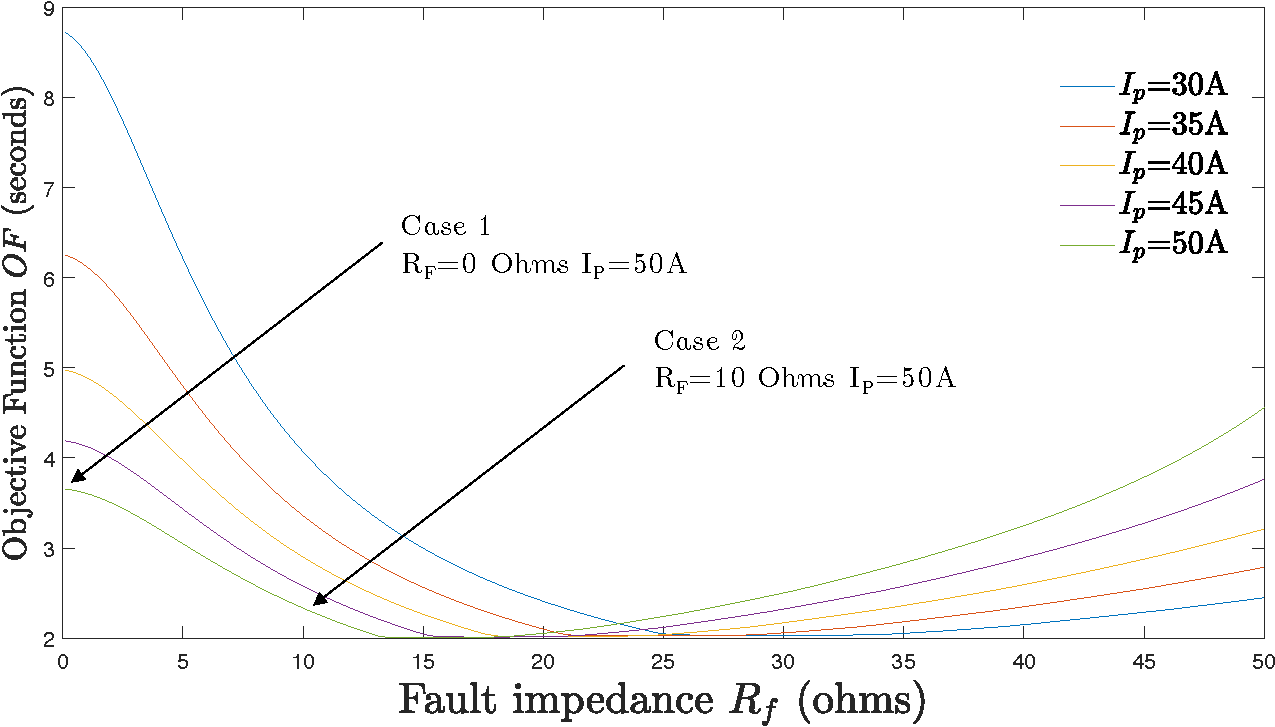
\includegraphics[width=9.0cm]{images/OF2.pdf}}
       \caption{Optimal clearing times  for  0$\le R_F \le$ 50 $\Omega$ and  30A$\le I_p \le$ 50A}
      \label{figure5}
        \end{figure}



\subsection{Sensitivity analysis }\label{3}

\textcolor{red}{When comparing cases 1 and 2 discussed above we can observe a decrease on both the objective function and time dial settings. Thus, if the fault impedance is steadily increased fro  0 ohms we can expect to find an impedance value that yield a minimum operation time. A sensitivity analysis  was carried out to verify this behavior by setting five pickup settings from 30A to 50A in steps of 5A, and by producing faults in a range 
between 0 ohms and $R_F$=50  $\Omega$ in steps of 0.1 $\Omega$.  Thus, 2500 optimization problems were solved. Figures 6 and t display the optimal operation time and the optimal relay time dial settings required to get minimum clearing times, respectively.}

 Figure 6 highlights the solutions reported in case 1 ($R_F$=0 $\Omega$, $I_p$=50A) and case 2 ($R_F$=10 $\Omega$, $I_p$=50A). The minimum value of the OF for $I_p$=50A is reached when $R_F$=14.9 $\Omega$ (OF = 2.005s). As seen in Fig.  6 this minimum value occurs when $D_2$=$D_5$=0.1.

  If we continue increasing $R_F$ from 15 $\Omega$ ($I_p$=50A) to 50 $\Omega$ ($I_p$=50A), the operation times (OF) steadily increases up to reach a maximum (4.22s for $R_F$=50  $\Omega$) with invariant optimal time dial settings). The fact that optimal time dial settings do not change from 17.5 up to 50 $\Omega$  implies that separation times will increase as far as the fault impedance also increases.  For $R_F>$50.0  $\Omega$ the optimization problem is not well defined due to sensitivity problems in some relay pairs and no efficient relay coordination is attainable.
           \begin{figure}[t!] \centerline{
           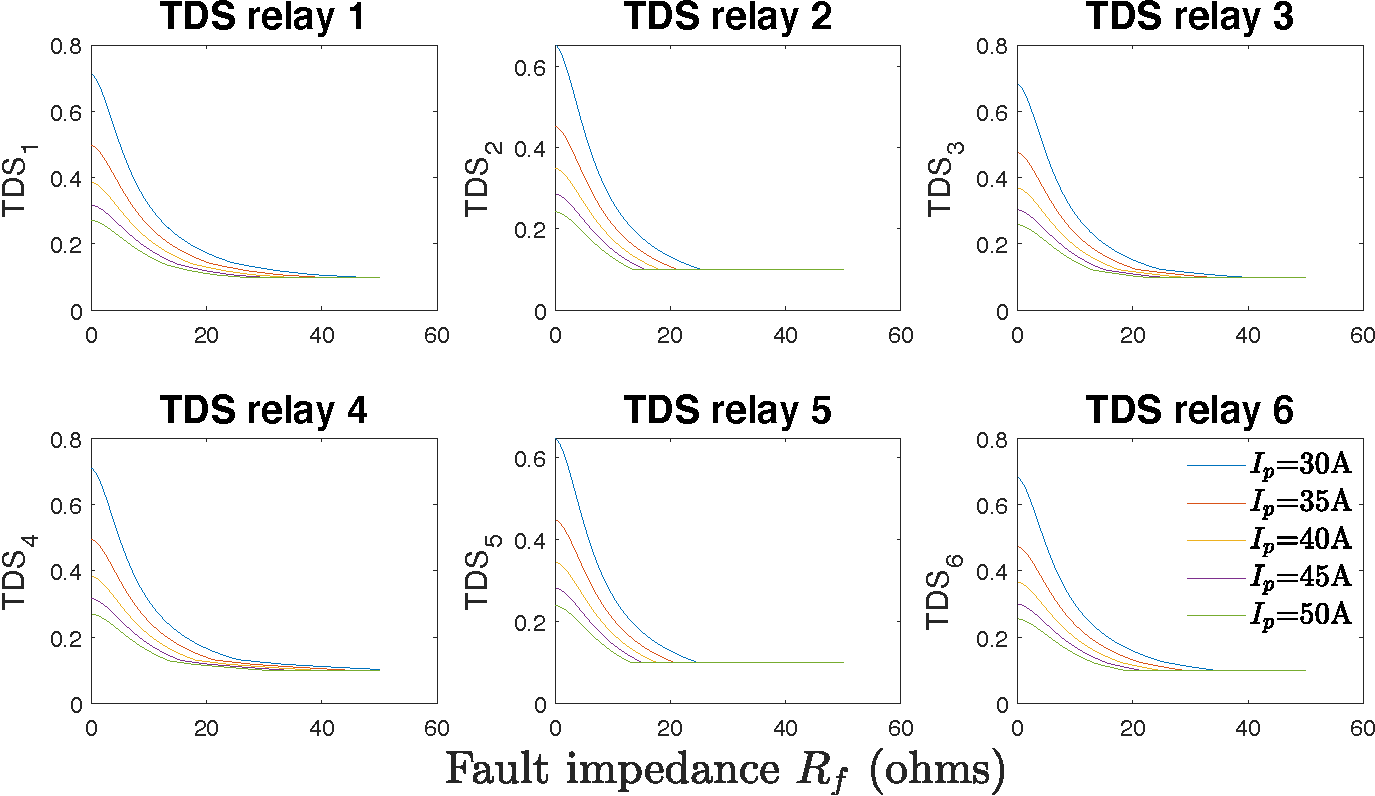
\includegraphics[width=9cm]{images/TDS2.pdf}}
       \caption{Optimal TDS for  0$\le R_F \le$ 50 $\Omega$ and  30A$\le I_p \le$ 50A}
      \label{figure6}
        \end{figure}

\textcolor{red}{Previous discussion was made on the assumption that the pickup current is set in 50A. If we reduce the pickups from 50 to 30A, we can observe  that the optimal operation times (OF, from Fig. 6) and the time dials (TDSs from Fig. 7) must higher to  address full selectivity. As a result, larger fault resistances are required to get the minimum objective function when the TDSs reach its minimum values. Beyond this point, when al TDSs are 0.1, the operation time (OF) deteriorates for all pickups.} 
 

\section{Conclusions and further research} \label{conclusions}

\textcolor{red}{In this paper we analyze how optimal operation times and selectivity regarded to optimal coordination of  neutral directional overcurrent relays are affected considering different impedance  fault magnitudes.} 

\textcolor{red}{Results show how the optimal operation time decreases as far as the fault impedance magnitude increases regardless the magnitude of pickup settings chosen by the protection engineer. When the fault impedance rises,  the optimized time dial settings also decreases stagnating at their minimum values. Beyond this point, the time dials are bounded and the clearing times deteriorate as far the fault impedance also increases.}

\textcolor{red}{We also find in this example that if the time dials are optimized by the protection engineer considering  the current practice (solid faults) but the fault type is really non-solid, the verification procedure shows shorter (better) relay operating times than the ones reported by the optimization procedure.}

\textcolor{red}{The main limitation of this work lies on the deterministic representation of the fault resistance. Future work must pose this problem as a stochastic optimization problem where all settings, time dial and pickup settings, are included in the mathematical model. Further efforts would be devoted to solve this problem considering a more realistic condition accounting transient configurations during the clearing time process. In this case, the use of near-end and far-end faults o setup the optimization model should not be enough to assure full selectivity}








 % \scriptsize
%\begin{verbatim}
%clear all
%New circuit.SOURCE_1a bus1=n1.1 bus2=n1.4
%basekV=39.84 pu=1 angle=0    Z1=[0,  9.50] basefreq=60 phase=1
%New Vsource.SOURCE_1b bus1=n1.2 bus2=n1.4
%basekV=39.84 pu=1 angle=-120 Z1=[0,  9.50] phase=1
%New Vsource.SOURCE_1c bus1=n1.3 bus2=n1.4
%basekV=39.84 pu=1 angle=120  Z1=[0,  9.50] phase=1
%New Vsource.SOURCE_2a bus1=n3.1 bus2=n2.4
%basekV=39.84 pu=1 angle=0    Z1=[0, 22.85] phase=1
%New Vsource.SOURCE_2b bus1=n3.2 bus2=n2.4
%basekV=39.84 pu=1 angle=-120 Z1=[0, 22.85] phase=1
%New Vsource.SOURCE_2c bus1=n3.3 bus2=n2.4
%basekV=39.84 pu=1 angle=120  Z1=[0, 22.85] phase=1
%New Vsource.SOURCE_3a bus1=n5.1 bus2=n3.4
%basekV=39.84 pu=1 angle=0    Z1=[0, 17.14] phase=1
%New Vsource.SOURCE_3b bus1=n5.2 bus2=n3.4
%basekV=39.84 pu=1 angle=-120 Z1=[0, 17.14] phase=1
%New Vsource.SOURCE_3c bus1=n5.3 bus2=n3.4
%basekV=39.84 pu=1 angle=120  Z1=[0, 17.14] phase=1
%set earthmodel=carson
%new wiredata.c1 Runits=mi Rac=0.2023 GMRunits=ft GMRac=0.02600
%new wiredata.c2 Runits=mi Rac=0.1756 GMRunits=ft GMRac=0.03210
%new wiredata.n  Runits=mi Rac=0.5920 GMRunits=ft GMRac=0.00814
%!!!! line 1-2
%new linegeometry.4wire12 nconds=4 nphases=3 reduce=no
%~ cond=1 wire=c2 units=ft x=5.5    h=40
%~ cond=2 wire=c2 units=ft x=5.5    h=50.6
%~ cond=3 wire=c2 units=ft x=5.5    h=61.2
%~ cond=4 wire=n  units=ft x=0      h=82.4
%!!!! line 1-3
%new linegeometry.4wire13 nconds=4 nphases=3 reduce=no
%~ cond=1 wire=c1 units=ft x=6    h=40
%~ cond=2 wire=c1 units=ft x=6    h=47.85
%~ cond=3 wire=c1 units=ft x=6    h=55.7
%~ cond=4 wire=n  units=ft x=0    h=71.4
%!!!! line 2-3
%new linegeometry.4wire23 nconds=4 nphases=3 reduce=no
%~ cond=1 wire=c2 units=ft x=5    h=40
%~ cond=2 wire=c2 units=ft x=5    h=49.7
%~ cond=3 wire=c2 units=ft x=5    h=59.4
%~ cond=4 wire=n  units=ft x=0    h=78.8
%new line.line11 geometry=4wire12 length=25
%units=km bus1=n1.1.2.3.4 bus2=n4.1.2.3.4  Rho=100
%new line.line12 geometry=4wire12 length=25
%units=km bus1=n4.1.2.3.4 bus2=n2.1.2.3.4  Rho=100
%new line.line21 geometry=4wire23 length=20
%units=km bus1=n2.1.2.3.4 bus2=n5.1.2.3.4  Rho=100
%new line.line22 geometry=4wire23 length=20
%units=km bus1=n5.1.2.3.4 bus2=n3.1.2.3.4  Rho=100
%new line.line31 geometry=4wire13 length=30
%units=km bus1=n3.1.2.3.4 bus2=n6.1.2.3.4  Rho=100
%new line.line32 geometry=4wire13 length=30
%units=km bus1=n6.1.2.3.4 bus2=n1.1.2.3.4  Rho=100
%!Reactors
%New Reactor.b1 Phases=1 Bus1=n1.4 Bus2=n1.0 R=000 X=0
%New Reactor.b2 Phases=1 Bus1=n2.4 Bus2=n2.0 R=000 X=0
%New Reactor.b3 Phases=1 Bus1=n3.4 Bus2=n3.0 R=000 X=0
%New Reactor.b4 Phases=1 Bus1=n4.4 Bus2=n4.0 R=0.5 X=0
%New Reactor.b5 Phases=1 Bus1=n5.4 Bus2=n5.0 R=0.5 X=0
%New Reactor.b6 Phases=1 Bus1=n6.4 Bus2=n6.0 R=0.5 X=0
%solve
%New fault.1n Bus1=n4.3 Bus2=n4.4 r=0.0001
%!New fault.1n Bus1=n5.3 Bus2=n5.4 r=0.0001
%!New fault.1n Bus1=n6.3 Bus2=n6.4 r=0.0001
%\end{verbatim}
%\normalsize


% \begin{IEEEbiography}
%    [{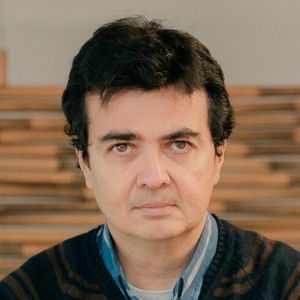
\includegraphics[width=1in,height=1.25in,clip,keepaspectratio]{images/paulo.jpg}}]{P. M. De Oliveira De Jesus}
%(M'03, SM'14) received the M.Sc. and the Electrical Engineering (5 year course) degree in 2002 and 1.995
%from Universidad Sim\'on Bol\'ivar (USB), Caracas, Venezuela, and
%Ph.D. (2008) degree from Oporto University, Portugal. Postdoctoral research at Coimbra University, Portugal in 2014-2015.  Former head of the USB's Energy Institute. Associate professor 2007-2014. Full professor2014-2016.
%Currently he
%is visiting professor with the Department
%of Electrical Engineering, School of Engineering,
%Universidad de Los Andes, Colombia. His
%research interests include technical and economic issues of electric
%power and energy systems.
%\end{IEEEbiography}
% 
% 
% 
%
%\begin{IEEEbiography}
%[{
\includegraphics[width=1in,height=1.25in,clip,keepaspectratio]{images/david.jpg}}]
%{D. F. Celeita} (SM'2019)
%received the degree in Electronic Engineering (2011) from Universidad Distrital Francisco José de Caldas, Bogotá, Colombia and M.Sc. (2014) and Ph.D (2018) in Electrical Engineering from Universidad de los Andes, Bogota, Colombia. He worked as an automation engineer in low and medium voltage applications for a few years. He was a visiting researcher at Georgia Institute of Technology and he served as a postdoctoral researcher at CentraleSupélec with an industry partner in France. He is currently a Postdoctoral Research Associate at Universidad de los Andes. His research interest includes Protective - Relaying Control, Smart Grids, Advanced Distribution Automation, Fault Location, and Real-Time Simulation.
%\end{IEEEbiography}
%
% \begin{IEEEbiography}
%    [{
\includegraphics[width=1in,height=1.25in,clip,keepaspectratio]{images/gustavo.jpg}}]{G.A. Ramos}
%(M'04 - SM'13)
%received the degree in Electrical
%Engineering (1997) from Universidad
%Nacional, Manizales, Colombia, and
%M.Sc. (1999) and PhD (2008) in
%Electrical Engineering from
%Universidad de Los Andes, Bogotá,
%Colombia. He is currently an Associate
%Professor with the Department of
%Electrical Engineering at School of
%Engineering, Universidad de Los Andes, Colombia where is
%involved in teaching courses on power electronics,
%fundamentals of power systems, power quality, distribution,
%and industrial systems design. His research interests include
%power quality and transients in grounding systems.\end{IEEEbiography}



\bibliographystyle{IEEEtran}
\bibliography{References2.bib}
\scriptsize
\textbf{P. M. De Oliveira De Jesus} (M'03 - SM'14) received the M.Sc. and the Electrical Engineering (5 year course) degree in 2002 and 1.995
from Universidad Sim\'on Bol\'ivar (USB), Caracas, Venezuela, and
Ph.D. (2008) degree from Oporto University, Portugal. Postdoctoral research at Coimbra University, Portugal in 2014-2015.  Former head of the USB's Energy Institute. Associate professor 2007-2014. Full professor2014-2016.
Currently he
is visiting professor with the Department
of Electrical Engineering, School of Engineering,
Universidad de Los Andes, Colombia. His
research interests include technical and economic issues of electric
power and energy systems.

\noindent\textbf{E. Sorrentino} received his Electrical Engineer (Cum Laude, 1984) and M.Sc. (Honors, 1986)
degrees from Universidad Sim\'on Bol\'ivar (USB,
Caracas, Venezuela), and his Ph.D. degree (Cum
Laude, 2014) from Universidad Carlos III de Madrid
(Spain). Since 1984, he has been a professor 
and a consulting engineer for several companies. His
research interests include power system protection,
power system analysis, and electrical machines.
 
 
\noindent\textbf{J.S. Abello}  has a
electrical engineer degree from the Universidad de los Andes (2019).
 
\noindent\textbf{O. Archilla} has a
electrical engineer degree from the Universidad de los Andes (2019).
 

 
\noindent\textbf{C. Alza}  has a
electrical engineer degree from the Universidad de los Andes (2019).
 
 
\noindent\textbf{D. F. Celeita } (SM'2019)
received the degree in Electronic Engineering (2011) from Universidad Distrital Francisco José de Caldas, Bogotá, Colombia and M.Sc. (2014) and Ph.D (2018) in Electrical Engineering from Universidad de los Andes, Bogota, Colombia. He worked as an automation engineer in low and medium voltage applications for a few years. He was a visiting researcher at Georgia Institute of Technology and he served as a postdoctoral researcher at CentraleSupélec with an industry partner in France. He is currently a Postdoctoral Research Associate at Universidad de los Andes. His research interest includes Protective - Relaying Control, Smart Grids, Advanced Distribution Automation, Fault Location, and Real-Time Simulation.


\noindent\textbf{G.A. Ramos} (M'04 - SM'13)
received the degree in Electrical
Engineering (1997) from Universidad
Nacional, Manizales, Colombia, and
M.Sc. (1999) and PhD (2008) in
Electrical Engineering from
Universidad de Los Andes, Bogot\'a�,
Colombia. He is currently an Associate
Professor with the Department of
Electrical Engineering at School of
Engineering, Universidad de Los Andes, Colombia where is
involved in teaching courses on power electronics,
fundamentals of power systems, power quality, distribution,
and industrial systems design. His research interests include
power quality and transients in grounding systems.


\noindent\textbf{A. J. Urdaneta }(SM'90) received the Elect. Eng. (Hons.) degree from the Universidad Sim\'on Bol\'ivar, Caracas, Venezuela, in 1979, the M.Sc. degree in electrical engineering and applied physics in 1983, and the Ph.D. degree in systems engineering in 1986, both from Case Western Reserve University, Cleveland, OH. Retired Professor of electrical engineering, Department of Energy Conversion and Delivery, Universidad Sim\'on Bol\'ivar. He has been responsible for a number of projects and studies performed for local industries. He is the former Dean of Professional Studies and former Chairman of the IEEE Venezuelan Section. His research interests are in the area of power system analysis and optimization. 

 

 
\end{document}
